\section{}

\subsection{Ni-Al system plotted using Thermo-Calc}

% First part
\begin{figure}[h]
    \centering
    \subfloat[Binary Ni-Al ASM Materials Handbook \label{fig:diagrama_ejemplo}]{
        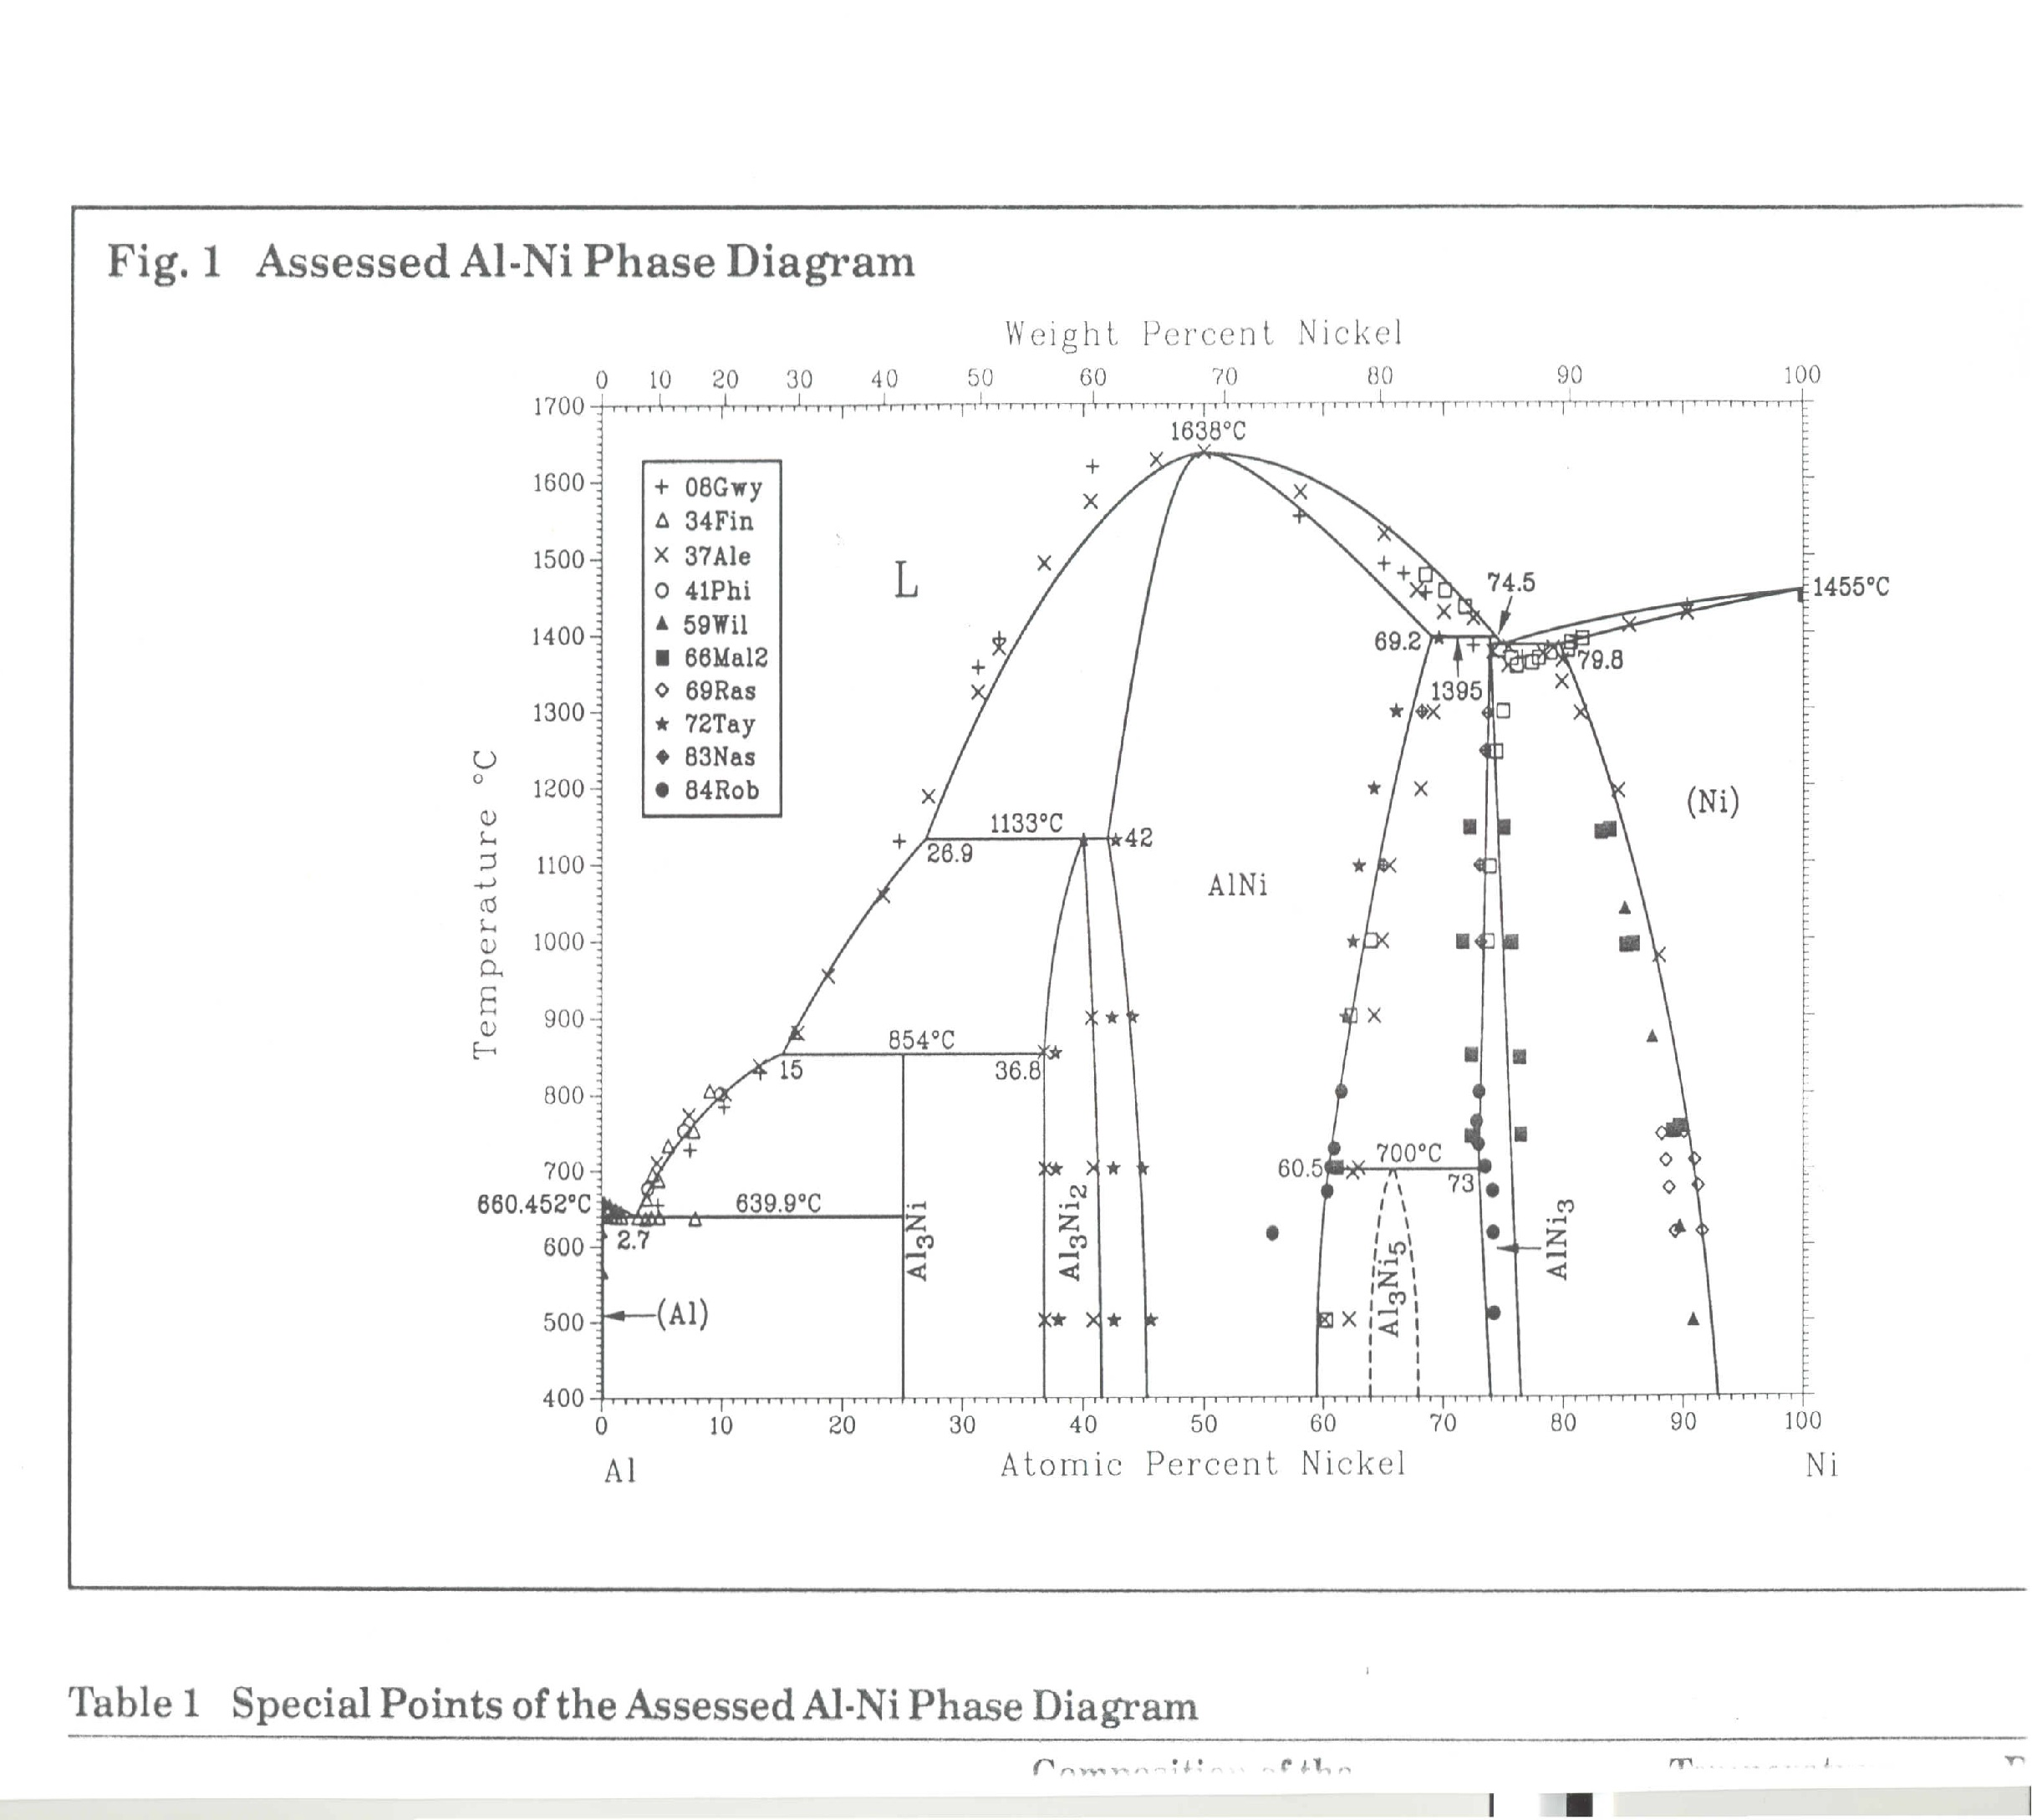
\includegraphics[width=0.85\textwidth]{graficas/diagrama_base.jpg}
        }
        \caption{Ni-Al binary phase diagram}
    \label{fig:Ni-Al_binarydiagram}
\end{figure}
% Second part (automatically continues numbering)
\begin{figure}[h]
    \centering
    \ContinuedFloat % This is the key command
    \subfloat[\centering Ni-Al system obtained using \textit{ThermoCalc} \citep{thermocalc} \label{fig:diagrama01}]{
        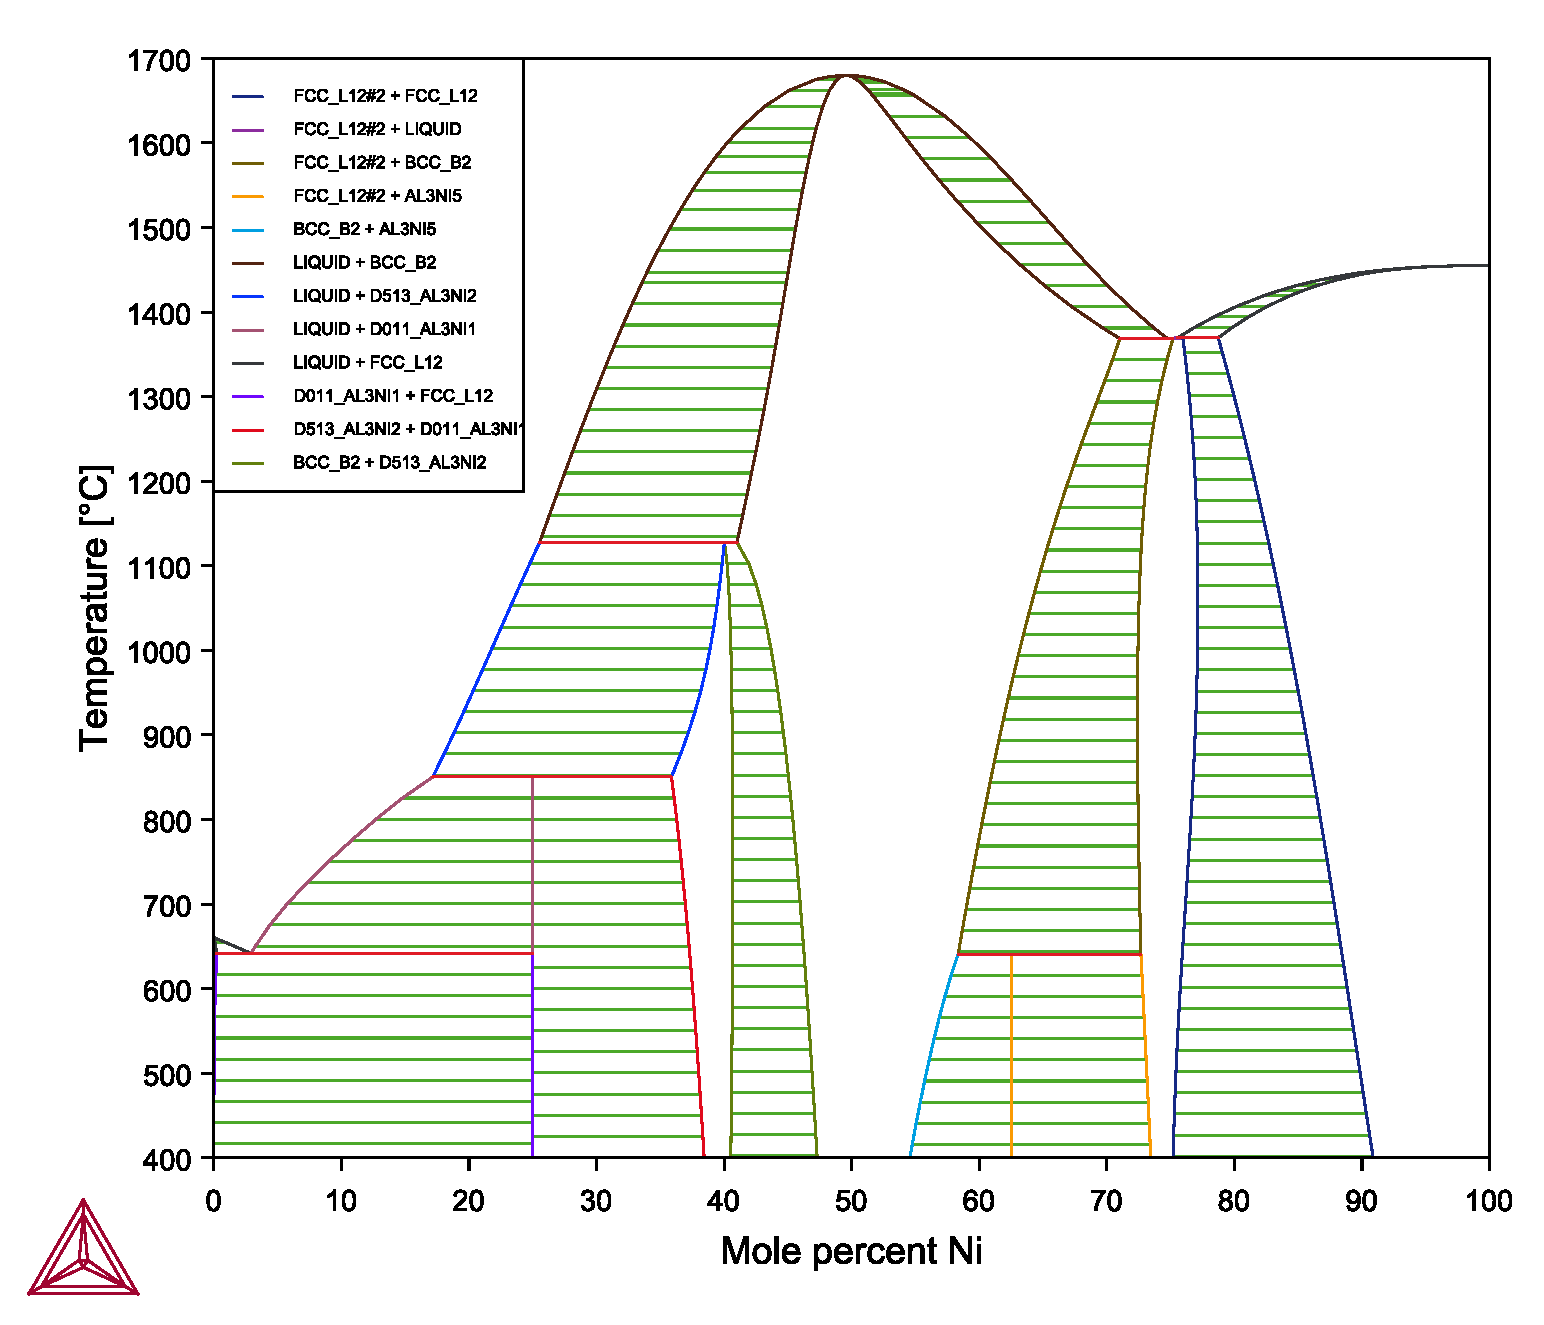
\includegraphics[width=0.9\textwidth]{graficas/Q1_NI_Al_binarydiagram.pdf}
        }
        \caption[]{Ni-Al binary phase diagram (continued)}
\end{figure}

Figure \ref{fig:diagrama_ejemplo} presents the binary phase diagram from the ASM Materials Handbook; and figure \ref{fig:diagrama01} presents the Ni-Al binary diagram obtained using \textit{ThermoCalc}, using the \textit{binary calculator} tool.

\newpage
\subsection{Composition of Al in Ni-Al system for a $\gamma'$ fraction is $75\%$. Target operating temperature $1000^{\circ}$C}

The composition of the $\gamma'$ phase was calculated using the \textit{single point} tool in \textit{ThermoCalc}, from which the following results were obtained:

\begin{table}[H]
    \centering
    \begin{tabular}{lrrr}
        \multicolumn{1}{c}{\textbf{Property}} & \multicolumn{1}{c}{\textbf{Value}} \\ \hline \hline
        Moles & 1 \\ 
        Mass (g) & 51.9841 \\ 
        Temperature (K) & 1273.15 \\ 
        Total Gibbs Energy (J) & -94721.9 \\
        Enthalpy (J) & -2475.10 \\
        Volume (m\textsuperscript{3}) & 0 \\ \\
        \multicolumn{1}{c}{\textbf{Component}} & \multicolumn{1}{c}{\textbf{Mole Fraction}} & \multicolumn{1}{c}{\textbf{Mass Fraction}} & \multicolumn{1}{c}{\textbf{Activity}}\\ \hline \hline
        Al & 0.211490 & 0.109773 & 1.13944E-08 \\
        Ni & 0.788510 & 0.890227 & 0.00159239
    \end{tabular}
    \caption{Results obtained from the calculation of the composition of the Ni-Al system for a $\gamma'$ phase at $75\%$ using \textit{ThermoCalc} \citep{thermocalc}}
    \label{tab:tab01}
\end{table}

From the results presented in table \ref{tab:tab01} it can be seen that for the $\gamma'$ wit a fraction of $75\%$ at $1000^{\circ}$C the composition for Al is $0.2115$ ($21.15\%$) mole fraction which is equivalent to a $10.98$ weight percent.